% Use this template to write your solutions to COS 423 problem sets

\documentclass[12pt]{article}
\usepackage[utf8]{inputenc}
\usepackage{amsmath, amsfonts, amsthm, amssymb, algorithm, graphicx, mathtools, xfrac}
\usepackage[noend]{algpseudocode}
\usepackage{fancyhdr, lastpage}
\usepackage{booktabs}
\usepackage{multirow}
\usepackage{graphicx}
\usepackage{pgfplots}
\usepackage[vmargin=1.20in,hmargin=1.25in,centering,letterpaper]{geometry}
\setlength{\headsep}{.50in}
\setlength{\headheight}{15pt}

% Landau notation
\DeclareMathOperator{\BigOm}{\mathcal{O}}
\newcommand{\BigOh}[1]{\BigOm\left({#1}\right)}
\DeclareMathOperator{\BigTm}{\Theta}
\newcommand{\BigTheta}[1]{\BigTm\left({#1}\right)}
\DeclareMathOperator{\BigWm}{\Omega}
\newcommand{\BigOmega}[1]{\BigWm\left({#1}\right)}
\DeclareMathOperator{\LittleOm}{\mathrm{o}}
\newcommand{\LittleOh}[1]{\LittleOm\left({#1}\right)}
\DeclareMathOperator{\LittleWm}{\omega}
\newcommand{\LittleOmega}[1]{\LittleWm\left({#1}\right)}

% argmin and argmax
\newcommand{\argmin}{\operatornamewithlimits{argmin}}
\newcommand{\argmax}{\operatornamewithlimits{argmax}}

\newcommand{\calP}{\mathcal{P}}
\newcommand{\Z}{\mathbb{Z}}
\newcommand{\R}{\mathbb{R}}
\newcommand{\Exp}{\mathbb{E}}
\newcommand{\Q}{\mathbb{Q}}
\newcommand{\sign}{\mathrm{sign\ }}
\newcommand{\abs}{\mathrm{abs\ }}
\newcommand{\eps}{\varepsilon}
\newcommand{\zo}{\{0, 1\}}
\newcommand{\SAT}{\mathit{SAT}}
\renewcommand{\P}{\mathbf{P}}
\newcommand{\NP}{\mathbf{NP}}
\newcommand{\coNP}{\co{NP}}
\newcommand{\co}[1]{\mathbf{co#1}}
\renewcommand{\Pr}{\mathop{\mathrm{Pr}}}

% theorems, lemmas, invariants, etc.
\newtheorem{theorem}{Theorem}
\newtheorem{lemma}[theorem]{Lemma}
\newtheorem{invariant}[theorem]{Invariant}
\newtheorem{corollary}[theorem]{Corollary}
\newtheorem{definition}[theorem]{Definition}
\newtheorem{property}[theorem]{Property}
\newtheorem{proposition}[theorem]{Proposition}

% piecewise functions
\newenvironment{piecewise}{\left \{\begin{array}{l@{,\ }l}}
{\end{array}\right.}

% paired delimiters
\DeclarePairedDelimiter{\ceil}{\lceil}{\rceil}
\DeclarePairedDelimiter{\floor}{\lfloor}{\rfloor}
\DeclarePairedDelimiter{\len}{|}{|}
\DeclarePairedDelimiter{\set}{\{}{\}}

\makeatletter
\@addtoreset{equation}{section}
\makeatother
\renewcommand{\theequation}{\arabic{section}.\arabic{equation}}

% algorithms
\algnewcommand\algorithmicinput{\textbf{INPUT:}}
\algnewcommand\INPUT{\item[\algorithmicinput]}
\algnewcommand\algorithmicoutput{\textbf{OUTPUT:}}
\algnewcommand\OUTPUT{\item[\algorithmicoutput]}


% Formating Macros

\pagestyle{fancy}
\lhead{\sc \hmwkClass\ $\; \;\cdot \; \;$ \hmwkSemester\ $\; \;\cdot \; \;$
Problem \hmwkAssignmentNum.\hmwkProblemNum}
%\chead{\sc Problem \hmwkAssignmentNum.\hmwkProblemNum}
%\chead{}
\rhead{\em \hmwkAuthorName\ $($\hmwkAuthorID$)$\/}
\cfoot{}
\lfoot{}
\rfoot{\sc Page\ \thepage\ of\ \protect\pageref{LastPage}}
\renewcommand\headrulewidth{0.4pt}
\renewcommand\footrulewidth{0.4pt}

\fancypagestyle{fancycollab}
{
    \lfoot{\textit{Collaborators: \hmwkCollaborators}}
}

\fancypagestyle{problemstatement}
{
    \rhead{}
    \lfoot{}
}

%%%%%% Begin document with header and title %%%%%%%%%%%%%%%%%%%%%%%%%

\begin{document}

%%%%%% Header Information %%%%%%%%%%%%%%%%%%%%%%%%%%%%%%%%%%%%%%%%%%%

%%% Shouldn't need to change these
\newcommand{\hmwkClass}{COS 255}
\newcommand{\hmwkSemester}{Spring 2016}

%%% Your name, in standard First Last format
\newcommand{\hmwkAuthorName}{Lukas Leung}
%%% Your NetID
\newcommand{\hmwkAuthorID}{lleung}

%%% The problem set number (just the number)
\newcommand{\hmwkAssignmentNum}{9}

%%% The problem number (just the number)
\newcommand{\hmwkProblemNum}{0}

%%% A list of your collaborators' NetIDs, separated by ", ".
%%% You can use a new line ("\\") in the middle to prevent a long
%%% list from overflowing.
\newcommand{\hmwkCollaborators}{}
%%% Sets the collaborator list to appear on the first page
\thispagestyle{fancycollab}

%%%%%%% begin Solution %%%%%%%%%%%%%%%%%%%%%%%%%%%%%%%%%%%%%%%%%%%%
\section*{Results from UVA}
\subsection{Problem A (page 2)}

\includegraphics[width=\textwidth]{ProblemA}
\subsection{Problem D (page 5)}
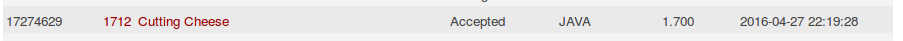
\includegraphics[width=\textwidth]{ProblemD}
\subsection{Problem E (page 9)}
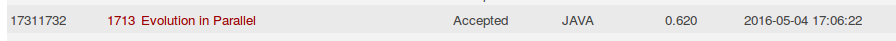
\includegraphics[width=\textwidth]{ProblemE}
\subsection{Problem F (page )}
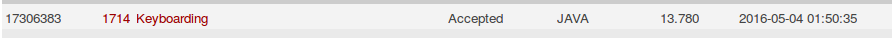
\includegraphics[width=\textwidth]{ProblemF}
\newpage

%%%%%%% start Problem A %%%%%%%%%%%%%%%%%%%%%%%%%%%%%%%%%%%%%%%%%%%

\section{Problem A: Amalgamated Artichokes}
\noindent \textbf{Results:} \\


\includegraphics[width=\textwidth]{ProblemA} \\

\noindent \textbf{Background:} \\
~\indent Fatima Cynara is an analyst at Amalgamated Artichokes (AA). As with any company, AA has had some
very good times as well as some bad ones. Fatima does trending analysis of the stock prices for AA, and she
wants to determine the largest decline in stock prices over various time spans. For example, if over a span
of time the stock prices were 19, 12, 13, 11, 20 and 14, then the largest decline would be 8 between the first
and fourth price. If the last price had been 10 instead of 14, then the largest decline would have been 10
between the last two prices. \\
\indent Fatima has done some previous analyses and has found that the stock price over any period of time can
be modelled reasonably accurately with the following equation:
\begin{center}$price(x) = p \cdot (sin(a\cdot x + b) + cos(c\cdot x + d) + 2)$\end{center}
where $p,a,b,c,\ and\ d$ are constants.Fatima would like you to write a program to determine the largest
price decline over a given sequence of prices. You have to consider the prices only for integer values of $x$. \\

\noindent \textbf{Input:} \\
~\indent The input file contains several test cases. Each test case is on a single line containing 6 integers,
$p\ (1 \leq p \leq 1000),\ a,\ b,\ c,\ d\ (0 \leq a,b,c,d \leq 1000),\ and\ n\ (1 \leq n \leq 10^6)$. The first
5 integers are described above. The sequence of stock prices to consider are $price(1), price(2),..., price(n).$ \\

\noindent \textbf{Output:} \\
~\indent For each test case, display the maximum decline in stock prices. If there is no decline, display the
number '0'. Your output should have an absolute or relative error of at most $10^{-6}$. \\

\noindent \textbf{Sample Input:} \\
42 1 23 4 8 10  \\
100 7 615 998 801 3  \\
100 432 406 867 60 1000  \\

\noindent \textbf{Sample Output:} \\
104.855110477  \\
0.00           \\
399.303813

%%%%%%% end Problem %%%%%%%%%%%%%%%%%%%%%%%%%%%%%%%%%%%%%%%%%%%%%%%

\newpage

%%%%%%% Mathematical Formulation %%%%%%%%%%%%%%%%%%%%%%%%%%%%%%%%%%
\subsection{Mathematical Formulation}
Given an input of integers $p, a, b, c, d,\ and\ n$, the formula
$f(x) = p\cdot (sin(a\cdot x + b) + cos(c\cdot x + d) + 2)$ where $x \in [1, n]$, determine the largest
decrease between the integer values $x_i, x_j$ where $i \textless j$ and $x_i \geq x_j$ and there does
not exist another pair $x_k, x_l$ where $k \textless l$ and $x_k \geq x_l$ but $x_k - x_l \textgreater x_i - x_j$.

%%%%%%% Algorithm %%%%%%%%%%%%%%%%%%%%%%%%%%%%%%%%%%%%%%%%%%%%%%%%%

\subsection{Solution}
The main functionality of this algorithm is to plug in each point keeping track of the highest seen point, $h$,
the lowest seen point occuring after $l$, and the largest difference, $d = h-l$. It should be noted that since
we are always taking the difference between the two values, we can factor out the $\cdot p$ as well as neglect
the +2 portions of the formula. Also, to cut down on run time, it works in the java system if you \% pi each of
the entries before putting them into the sine and cosine functions. For whatever reason the larger the input,
the more costly the operation is.

\begin{algorithm}[H]
\caption{Main}
\begin{algorithmic}
    \Procedure{f}{x}
        \State $ab \gets$ (a*x+b) \% pi,
        \State $cd \gets$ (c*x+d) \% pi;
        \State return (Math.sin(ab) + Math.cos(cd))
    \EndProcedure
    \Procedure{Solve}{p, a, b, c, d, n}
        \State $val, h, l \gets$ f(1); $diff \gets$ 0
        \For{x $\in$ [2, n]} // if n = 1, do not execute
            \State $val \gets$ f(x)
            \If{$val \textgreater h$} // higher than current highest
                \State $h, l \gets$ val;
            \ElsIf{$val \textless l$} // lower than current lowest
                \State $l \gets$ val; $curDiff \gets$ h - l;
                \If{$curDiff \textgreater diff$}
                    $diff \gets$ curDiff;
                \EndIf
            \EndIf
        \EndFor
        \State \Call{print}{$p\cdot diff$}
    \EndProcedure
\end{algorithmic}
\end{algorithm}


%%%%%%% Correctness %%%%%%%%%%%%%%%%%%%%%%%%%%%%%%%%%%%%%%%%%%%%%%%

\subsection{Correctness}
%%%%%%% PROPOSITION 1 %%%%%%%%%%%%%%%
\begin{proposition}
~ \\ \indent We will determine the value of largest price decline over the interval $[1, n]$,
only considering $f(1), f(2),..., f(n)$.
\end{proposition}

\begin{proof}
~ \\ \indent We do this by keeping track of the largest price decline seen thus far, $diff$,
the current highest point seen, $h = f(x_i)$, and the current lowest point seen, $l = f(x_j)$,
such that $x_i \leq x_j,\ and\ f(x_i) \geq f(x_j)$. Therefore whenever we see a higher point,
$f(x_k) \textgreater f(x_i), x_k \textgreater x_i$, we update our $h = f(x_k)$ and reset our
lowest point to be $l = h$ since we are searching for the largest decline $\implies l$ must
occur \underline{after} $h$. Now every time that we see a number $f(x_m) \leq l$, we update
$l$ and check to see if our $h - l \geq diff$, if so we update diff, else we continue to the
next point.  If we see a higher point than $h$ we will repeat this process. Therefore we will
be looking at each subsequent highest correspoing following lowest points $\implies$ we will
see this largest price decline.
\end{proof}


%%%%%%% Analysis %%%%%%%%%%%%%%%%%%%%%%%%%%%%%%%%%%%%%%%%%%%%%%%%%%
\subsection{Analysis}

%%%%%%% PROPOSITION 1 %%%%%%%%%%%%%%%
\begin{proposition}
\label{numq}
The \underline{space complexity} of this algorithm is \textbf{O(1)}
\end{proposition}

\begin{proof}
~ \\ \indent This is due to the fact that we will only store the values $p, a, b, c, d, n, and diff$
as integer variables O(1):
\begin{center}
    Giving us a space complexity of \textbf{O(1)}
\end{center}
\end{proof}

%%%%%%% PROPOSITION 2 %%%%%%%%%%%%%%%
\begin{proposition}
\label{numq}
The \underline{time complexity} of this algorithm is \textbf{O(N)}
\end{proposition}

\begin{proof}
This is the case because our algorithm goes through the points $1, 2, ..., n$ once and only
calculates each value one time.
\begin{center}
    Giving us a time complexity of \textbf{O(N)}
\end{center}
\end{proof}

%%%%%%% Example %%%%%%%%%%%%%%%%%%%%%%%%%%%%%%%%%%%%%%%%%%%%%%%%%%%

\subsection{An Example}
Given the input of: \underline{42 1 23 4 8 10}, we will read this in as
$p = 42, a = 1, b = 23, c = 4, d = 8, and\ n = 10$. Then we will initialize our $h = l = f(1)$ and $diff = 0$.
Then starting with the second point until the 10th we will read through and record the values of what h, l, curDiff,
and diff are:

\begin{table}[H]
	\centering
	\resizebox{\textwidth}{!}{
	\begin{tabular}{c||c|c|c|c|c|c|c|c|c|c|}
		\toprule
		x =      & 1        & 2         & 3         & 4         & 5         & 6         & 7         & 8         & 9         & 10        \\
		\midrule
		f(x)    & -0.061724 & -1.090011 & 1.170641  & 1.380555  & -0.691700 & 0.170589  & -1.115995 & -1.070976 & 1.551270  & 0.359768 \\
        h       & -0.061724 & -0.061724 & 1.170641  & 1.380555  & 1.380555  & 1.380555  & 1.380555  & 1.380555  & 1.551270  & 1.551270 \\
        l       & -0.061724 & -1.090011 & 1.170641  & 1.380555  & -0.691700 & -0.691700 & -1.115995 & -1.115995 & 1.551270  & 0.359768 \\
        curDiff & --        & 1.028286  & --        & --        & 2.072255  & --        & 2.496550  & --        & --        & 1.191502 \\
        diff    & 0         & 1.028286  & 1.028286  & 1.028286  & 2.072255  & 2.072255  & 2.496550  & 2.496550  & 2.496550  & 2.496550 \\
        \bottomrule
	\end{tabular}}
\end{table}

Now multiplying our $diff$ by $p \implies 2.496550 \cdot 42 = 104.855110$ which is our solution.
%%%%%%% end Problem A %%%%%%%%%%%%%%%%%%%%%%%%%%%%%%%%%%%%%%%%%%%%%
\newpage
















%%%%%%% start Problem D %%%%%%%%%%%%%%%%%%%%%%%%%%%%%%%%%%%%%%%%%%%

\section{Problem D: Cutting Cheese}
\noindent \textbf{Results:} \\

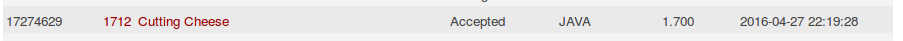
\includegraphics[width=\textwidth]{ProblemD} \\

\noindent \textbf{Background:} \\
~\indent Of course you have all heard of the International Cheese Processing Company. Their machine for cutting a piece
of cheese into slices of exactly the same thickness is a classic. Recently they produced a machine able to cut
a spherical cheese (such as Edam) into slices -- no, not all of the same thickness, but all of the same weight!
But new challenges lie ahead: cutting Swiss cheese. \\
\indent Swiss cheese such as Emmentaler has holes in it, and the holes may have different sizes.  A slice with
holes contains less cheese and has a lower weight than a slice without holes. So here is the challenge: cut a
cheese with holes in it into slices of equal weight. \\
\indent By smart sonar techniques (the same techniques used to scan unborn babies and oil  elds), it is possible
to locate the holes in the cheese up to micrometer precision. For the present problem you may assume that the
holes are perfect spheres. \\
\indent Each uncut block has size $100 x 100 x 100$ where each dimension is measured in millimeters. Your
task is to cut it into $s$ slices of equal weight. The slices will be $100 mm$ wide and $100 mm$ high, and
your job is to determine the thickness of each slice. \\

\noindent \textbf{Input:} \\
The input  le contains several test cases, each of them as described below: \\
\indent The first line of the input contains two integers $n$ and $s$, where $0 \leq n 10000$ is the number of
holes in the cheese, and $1 \leq s \leq 100$ is the number of slices to cut. The next $n$ lines each contain four
positive integers, $r, x, y,\ and\ z$ are the coordinates of the center, all in micrometers. The cheese block
occupied the points ($x, y, z$) where $0 \leq x, y, z \leq 100000$, except for the points that are part of
some hole. The cuts are made perpendicular to the z-axis. \\
\indent You may assume that holes do not overlap but may touch, and that the holes are fully contained
in the cheese but may touch its boundary. \\

\noindent \textbf{Output:} \\
~ \indent For each test case, display the s slice thicknesses in millimeters, starting from the end of the cheese
with $z = 0$. Your output should have an absolute or relative error of at most $10^{-6}$.



%%%%%%% end Problem %%%%%%%%%%%%%%%%%%%%%%%%%%%%%%%%%%%%%%%%%%%%%%%

\newpage

%%%%%%% Mathematical Formulation %%%%%%%%%%%%%%%%%%%%%%%%%%%%%%%%%%
\subsection{Mathematical Formulation}
Given an input of $n$ totally encapsulated, non-overlapping spheres, each with a $x$ position and $r$, radius we
can determine where to make cuts in a block of cheese 100000 x 100000 x 100000

%%%%%%% Algorithm %%%%%%%%%%%%%%%%%%%%%%%%%%%%%%%%%%%%%%%%%%%%%%%%%

\subsection{Solution}
~\indent The main functionality of this algorithm is to compute the total volume of the block of cheese, then determine
what the weight should be of each equally sliced piece and perform a binary search of segments (from the left
side, $z = 0$) to find the segments which are within $10^{-6}$ of this target weight. We calculate the volumes
of each block by using spherical segment calculations of all spheres within the range in question. \\
\indent The only data structure we used was a two dimentional array \textbf{holes$[n][2]$} such that
each entry $holes[i][0]$ corresponds to the center $z$ coordinate and $holes[i][1]$ is the radius of hole $i$.
Asside from this we use the instance variable $v, goal, numHoles, numSlices$ to keep track of the total volume,
the goal weight for evenly cut slices of cheese, the number of holes and the number of slices.

\begin{algorithm}[H]
\caption{Main}
\begin{algorithmic}
    \Procedure{main}{}
        \State $v, numHoles, numSlices, holes[numHoles][2] \gets$ initialized
        \For{hole $i \in [1..numHoles]$}
            \State store $i_z, i_r$ in index $i$
            \State update $v$
        \EndFor
        \State $goal \gets v/numSlices$
        \State Sort($holes$) based off of left-most point on sphere on z-axis
        \State \Call{binarySearch}{ }
    \EndProcedure
    \Procedure{binarySearch}{}
        \State (double) $low, high, last, cut \gets$ 0, 100000, 0.0
        \State (int) $slicePerformed \gets$ 1
        \While{true}
            \State $cut \gets$ $(h + l)/2$
            \State (double) $diff \gets$ goal - \Call{allVol}{last, cut}
            \If{$diff == 0$}
                \State \Call{print}{(cut-last)/1000}
                \State $last \gets call$; $l \gets last$; $h \gets 100000$;
                \If{slicePerformed++ == numSlices-1}
                    break;
                \EndIf
            \ElsIf{goal - val $\textgreater$ 0}
                $l \gets cut$
            \Else
                $h \gets cut$
            \EndIf
        \EndWhile
        \State \Call{print}{(100000 - last)/1000};
    \EndProcedure
\end{algorithmic}
\end{algorithm}

Since we have sorted by left most part of each sphere, as soon as the leftmost point of the $i^{th}$
hole is past the mark $b$, then the points $j \geq i$ are not contained in the bounds so we can break
out of the loop and not calculate any more spheres. Otherwise we calculate the spherical segments of
each sphere for which there is some portion of it in the band $[a,b]$. The link for equations used
can be found here: http://mathworld.wolfram.com/SphericalSegment.html.

\begin{algorithm}[H]
\caption{Computations}
\begin{algorithmic}
    \Procedure{allVol}{double a, double b}
        \State $vol \gets DIM\cdot DIM\cdot (b-a)$
        \For{$i \in 1..numHoles$}
            \If{$i_z - i_r \textgreater$ b}
                break;
            \EndIf
            \If{$i_z + i_r \textless$ a}
                continue;
            \EndIf
            \State $val -=$ \Call{volInRange}{a, b, i};
        \EndFor
        \State return $val$;
    \EndProcedure
    \Procedure{volInRange}{double a, double b, int i}
        \State Computes the spherical segment based off of the formulas in the link above.
    \EndProcedure
\end{algorithmic}
\end{algorithm}

%%%%%%% Correctness %%%%%%%%%%%%%%%%%%%%%%%%%%%%%%%%%%%%%%%%%%%%%%%

\subsection{Correctness}
\begin{corollary}
~ \\ \indent It is sufficient for us to simply view the spheres on a 1-dimentional plane because we are
ensured that each sphere is fully encapsulated within the block of cheese and that no two spheres are
overlapping, therefore if we take the band of [a,b], if some potion of sphere $i$ is within this we can
calcuate the volume displaced using only the portion $(i_a, i_b)$ that overlaps with sphere $i$ and its
radius, $i_r$.
\end{corollary}
%%%%%%% PROPOSITION 1 %%%%%%%%%%%%%%%
\begin{proposition}
~ \\ \indent Given the correct process for determining the volume of portions of spheres, a binary search
for cuts in the cheese will give us the correct cuts to make.
\end{proposition}

\begin{proof}
~ \\ \indent We know that binary search is a viable option for when we know the stopping criteria and
can calcualte or lookup each intermediate stage. Therefore if we perform $s$ binary searches, decreasing
our range appropriately each time we find a cut, and we know our stopping criteria as $goal$; we can
calcualte the volume displaced by each portion of a sphere in intemediate ranges $[a,b]$, ultimately
giving us the appropriate cut coordinates along the z-axis.
\end{proof}

\newpage
%%%%%%% Analysis %%%%%%%%%%%%%%%%%%%%%%%%%%%%%%%%%%%%%%%%%%%%%%%%%%
\subsection{Analysis}

%%%%%%% PROPOSITION 1 %%%%%%%%%%%%%%%
\begin{proposition}
\label{numq}
The \underline{space complexity} of this algorithm is \textbf{O(N)}
\end{proposition}

\begin{proof}
~ \\ \indent This is due to the fact that all we store are the z-coordinate and the radius of
each hole.
\begin{center}
    Giving us a space complexity of \textbf{O(N)}
\end{center}
\end{proof}

%%%%%%% PROPOSITION 2 %%%%%%%%%%%%%%%
\begin{proposition}
\label{numq}
The \underline{time complexity} of this algorithm is \textbf{O(N$\cdot$log(N) + N$\cdot$S$\cdot$log(S))}
\end{proposition}

\begin{proof}
This is the case because our initial sorting of the holes takes $N\cdot log(N)$, then within the binary
search ($S\cdot log(S)$) we do at most (worstcase if every interval contains every hole) $N$ volume
calculations.
\begin{center}
    Giving us a time complexity of \textbf{O(N$\cdot$log(N) + N$\cdot$S$\cdot$log(S))}
\end{center}
\end{proof}

%%%%%%% Example %%%%%%%%%%%%%%%%%%%%%%%%%%%%%%%%%%%%%%%%%%%%%%%%%%%

\subsection{An Example}
Given the input of:  \\
1 2                         \\
10000 10000 10000 50000     \\

Which is asking for 2 slices with one hole positioned at (x, y, z) = (10000, 10000, 50000) and the
radius is 10000. As we read in we learn:
\begin{center}$vol = 9.958112\cdot10^{14} \implies goal = 4.979056\cdot10^{14}$.\end{center}
For this case we record everything and make our initial cut at 50000, for which we calculate the sphere
takes up 2.094395$\cdot10^{12}$ $micrometers^3$ which gives us our goal of $4.979056\cdot10^{14}$. Therefore
we print out:
\begin{center}50.000000 \\
50.000000\end{center}

%%%%%%% end Problem D %%%%%%%%%%%%%%%%%%%%%%%%%%%%%%%%%%%%%%%%%%%%%
\newpage














%%%%%%% start Problem E %%%%%%%%%%%%%%%%%%%%%%%%%%%%%%%%%%%%%%%%%%%

\section{Problem E: Evolution}
\noindent \textbf{Results:} \\

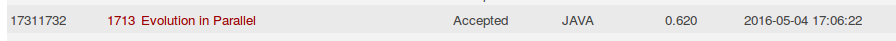
\includegraphics[width=\textwidth]{ProblemE} \\

\noindent \textbf{Background:} \\
~\indent  It is 2178, and alien life has been discovered on a distant planet. There seems to be only one species on
the planet and they do not reproduce as animals on Earth do. Even more amazing, the genetic makeup of every single
organism is identical! \\
\indent The genetic makeup of each organism is a single sequence of nucleotides. The nucleotides come in
three types, denoted by `A' (Adenine), `C' (Cytosine), and `M' (Muamine). According to one hypothesis,
evolution on this planet occurs when a new nucleotide is inserted somewhere into the genetic sequence
of an existing organism. If this change is evolutionarily advantageous, then organisms with the new
sequence quickly replace ones with the old sequence. \\
\indent It was originally thought that the current species evolved this way from a single, very simple
organism with a single-nucleotide genetic sequence, by way of mutations as described above. However,
fossil evidence suggests that this might not have been the case. Right now, the research team you are
working with is trying to validate the concept of "parallel evolution" -- that there might actually have
been two evolutionary paths evolving in the fashion described above, and eventually both paths evolved
to the single species present on the planet today. Your task is to verify whether the parallel evolution
hypothesis is consistent with the genetic material found in the fossil samples gathered by your team. \\

\noindent \textbf{Input:} \\
The input file contains several test cases, each of them as described below. \\
\indent The input begins with a number $n, (1 \leq n \leq 4000)$ denoting the number of nucleotide sequences
found in the fossils. The second line describes the nucleotide sequence of the species currently living
on the planet. Each of the next $n$ lines describes one nucleotide sequence found in the fossils. \\
\indent Each nucleotide sequence consists of a string of at least one but no more than 4 000 letters. The
strings contain only upper-case letters 'A', 'C', and 'M'. All the nucleotide sequences, including that of
the currently live species, are distinct. \\

\noindent \textbf{Output:} \\
~ \indent For each test case, display an example of how the nucleotide sequences in the fossil record participate in
two evolutionary paths. The example should begin with one line containing two integers $s_1$ and $s_2$, the
number of nucleotide sequences in the fossil record that participate in the first path and second path,
respectively. This should be followed by $s_1$ lines containing the sequences attributed to the first path,
in chronological order (from the earliest), and then $s_2$ lines containing the sequences attributed to the
second path, also in chronological order. If there are multiple examples, display any one of them. If
it is possible that a sequence could appear in the genetic history of both species, your example should
assign it to exactly one of the evolutionary paths. \\
\indent If it is impossible for all the fossil material to come from two evolutionary paths, display the word
'impossible'.



%%%%%%% end Problem %%%%%%%%%%%%%%%%%%%%%%%%%%%%%%%%%%%%%%%%%%%%%%%

%%%%%%% Mathematical Formulation %%%%%%%%%%%%%%%%%%%%%%%%%%%%%%%%%%
\subsection{Mathematical Formulation}
Given a currently present string $s_g$ and $N$ strings of average length $S$, determine if the $N$ strings can be
grouped into 2 sequences of evolutionary paths $sub_1$ and $sub_2$. A valid evolutionary path constitutes of having
each string to be a sub-sequence [defined below] of the proceeding string. Both $sub_1$ and $sub_2$ should be
sub-sequences of $s_g$ and if there is a string which does not belong to either $sub_1$ or $sub_2$ or they are not
a sub-sequence of $s_g$, then the algorithm will return "impossible".


%%%%%%% Algorithm %%%%%%%%%%%%%%%%%%%%%%%%%%%%%%%%%%%%%%%%%%%%%%%%%
\newpage
\subsection{Solution}
~\indent The main functionality of this algorithm is to first order the given strings in ascending order in terms
of length of string. Then we will build $sub_1$ and $sub_2$ top down, first appending $s_g$ then ensuring that every
subsequent string added to either $sub_1$ or $sub_2$ must be a sub-sequence [see helpers section for this] of the
currently smallest length element on them.

\begin{algorithm}[H]
\caption{Main}
\begin{algorithmic}
    \Procedure{main}{}
        \For{each test case}
            \State \Call{initialize}{} // see below
            \State boolean $failed, shared \gets$ false; String $lastS_1, lastS_2 \gets$ initialized
            \State $sub_1$.\Call{push}{$s_g$}; $sub_2$.\Call{push}{$s_g$};
            \For{each string $i$ from N..1}
                \State $token \gets$ sequence[i]
                \If{shared}
                    \If{isSubSequence(token, sharedList.peekFirst())}
                        \State sharedList.addFirst(token);
                    \ElsIf{isSubSequence(token, $lastS_1$)}
                        \State $sub_1$.\Call{push}{$token$}
                        \State $sub_2$.\Call{push}{sharedList}
                        \State $shared \gets$ true;
                    \ElsIf{isSubSequence(token, $lastS_2$)}
                        \State $sub_2$.\Call{push}{$token$}
                        \State $sub_1$.\Call{push}{sharedList}
                        \State $shared \gets$ true;
                    \Else
                        $failed \gets$ true
                    \EndIf
                \Else
                    \State (boolean) $inS_1, inS_2 \gets$ isSubSequence(token, $sub_{1,2}$.peek())
                    \If{$inS_1 \&\& inS_2$}
                        \State $shared \gets$ true; $lastS_1, lastS_2\gets sub_{1,2}$.peek();
                        \State sharedList.\Call{addFirst}{token}
                    \ElsIf{$inS_1$}
                        $sub_1$.\Call{push}{$token$}
                    \ElsIf{$inS_2$}
                        $sub_2$.\Call{push}{$token$}
                    \Else
                        $failed \gets$ true
                    \EndIf
                \EndIf
            \EndFor
            \If{failed}
                print("impossible");
            \Else
                \If{shared}
                    $sub_1$.\Call{push}{sharedList}
                \EndIf
                \State print($sub_1$.size() $sub_2$.size()); print($sub_1$); print($sub_2$);
            \EndIf
        \EndFor
    \EndProcedure
\end{algorithmic}
\end{algorithm}
\newpage
A string, $s_1$ is called a sub-sequence of $s_2$ if every letter in $s_1$ is present in $s_2$ and they occur
in the same order (though there can be different letters in between them).

\begin{algorithm}[H]
\caption{Helpers}
\begin{algorithmic}
    \Procedure{isSubSequence}{String $s_1$, String $s_2$}
        \State (int) $i \gets$ 0
        \For{$j \in [0..s_2.length]$}
            \If{$s_1$.charAt(i) == $s_2$.charAt(j)}
                \If{++i == $s_2$.length()}
                    return true;
                \EndIf
            \EndIf
        \EndFor
        \State return false;
    \EndProcedure
    \Procedure{initialize}{ }
        \State $N \gets$ number of strings; $sequence[N] \gets$ initialized and filled;
        \State $s_g \gets$ goal string (currently present string)
        \State \Call{sort}{sequence} by acending order
        \State Stack$\textless$String$\textgreater$ $sub_1, sub_2 \gets$ initialized;
        \State LinkedList$\textless$String$\textgreater$ $sharedList \gets$ initialized;
    \EndProcedure
\end{algorithmic}
\end{algorithm}

%%%%%%% Correctness %%%%%%%%%%%%%%%%%%%%%%%%%%%%%%%%%%%%%%%%%%%%%%%

\subsection{Correctness}
%%%%%%% PROPOSITION 1 %%%%%%%%%%%%%%%
\begin{proposition}
~ \\ \indent Given
\end{proposition}

\begin{proof}
~ \\ \indent We know that
\end{proof}

%%%%%%% Analysis %%%%%%%%%%%%%%%%%%%%%%%%%%%%%%%%%%%%%%%%%%%%%%%%%%
\subsection{Analysis}
Here we will refer to $N$ being number of strings inputed and $S$ as the average length of all the strings.
%%%%%%% PROPOSITION 1 %%%%%%%%%%%%%%%
\begin{proposition}
\label{numq}
The \underline{space complexity} of this algorithm is \textbf{O(N$\cdot$S)}
\end{proposition}

\begin{proof}
~ \\ \indent This is due to the fact that we store every string in our $sequence[N]$, our two stacks,
and the queue. Worst case the sum of the sizes of the two stacks and the queue will be $N$ becasue each string
is only present at one at a time. Therefore, since each of these contain every string, it becomes $S\cdot (N + N)$.
\begin{center}
    Giving us a space complexity of \textbf{O(N$\cdot$S)}
\end{center}
\end{proof}

%%%%%%% PROPOSITION 2 %%%%%%%%%%%%%%%
\begin{proposition}
\label{numq}
The \underline{time complexity} of this algorithm is \textbf{O(N$\cdot$log(N) + N$\cdot$S)}
\end{proposition}

\begin{proof}
This is the case because we first sort all of the strings based off of length ($N\cdot log(N)$). Then we will
perform the $isSubSequence$ method on each string a maximum of 4 times. Twice to determine sub for the top of
$s_1$ and $s_2$ then possibly to the string that may be place on top of it and then possibly again if they are
the end of a split as described in the proof above therefore giving us $N\cdot4\cdot S$ as worst case.

\begin{center}
    Giving us a time complexity of \textbf{O(N$\cdot$log(N) + N$\cdot$S)}
\end{center}
\end{proof}

%%%%%%% Example %%%%%%%%%%%%%%%%%%%%%%%%%%%%%%%%%%%%%%%%%%%%%%%%%%%

\subsection{An Example}
Given the input of:  \\

%%%%%%% end Problem E %%%%%%%%%%%%%%%%%%%%%%%%%%%%%%%%%%%%%%%%%%%%%

%%%%%%% end Solution %%%%%%%%%%%%%%%%%%%%%%%%%%%%%%%%%%%%%%%%%%%%%%

\end{document}